\subsection{zweites}
\[
  P_b=t\partial_t^2+2\partial_t-1
\]

$
P_b=t\partial_t^2+2\partial_t-1 \Rightarrow 
\begin{cases}
  k=2,l=1 & \Rightarrow u\leq k=2, v\geq l-k=-1\\
  k=1,l=0 & \Rightarrow u\leq 1, v\geq -1\\
  k=0,l=0 & \Rightarrow u\leq 0, v\geq 0\\
\end{cases}
$

\begin{center}
  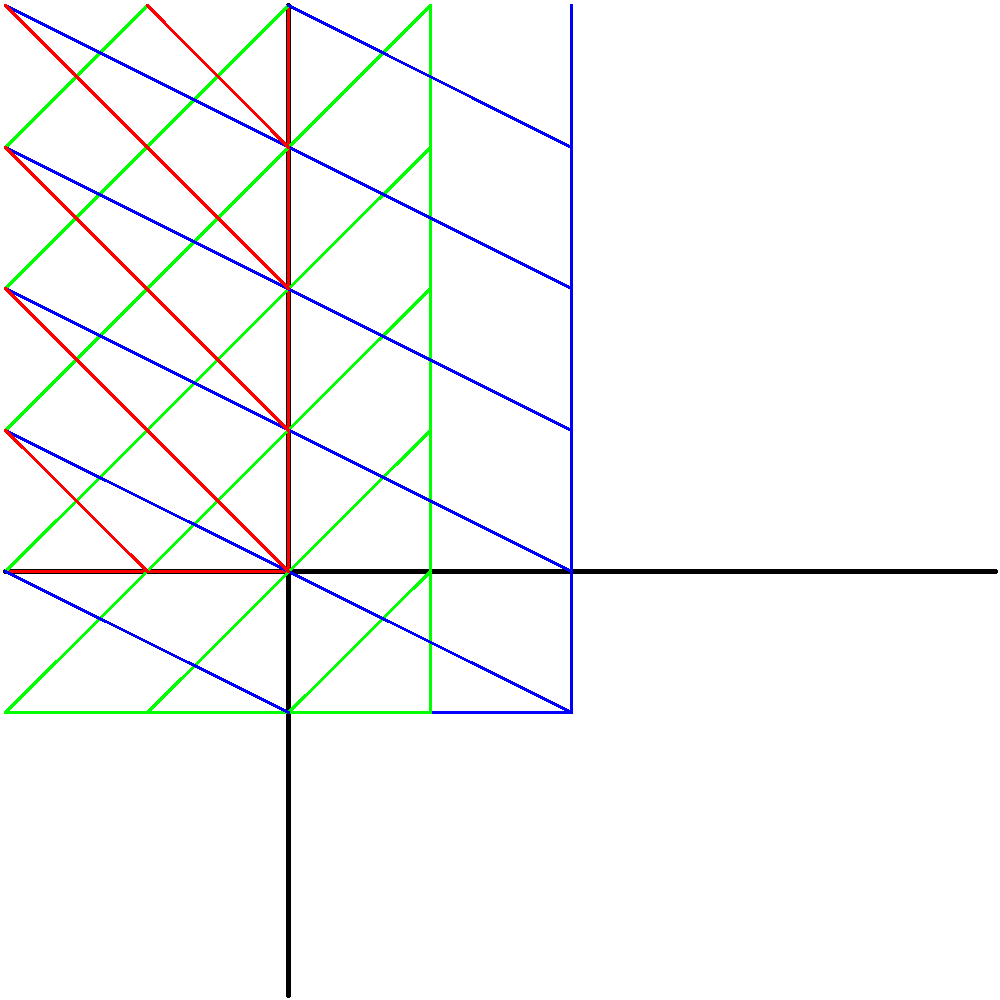
\includegraphics[width=6cm]{img/b.png}
\end{center}
also $\slopes(P_b)=\{0\}$ also ist $P_b$ regulär singulär

% vim: set ft=tex :
